% Plantilla creada originalmente por la Dra. BEeatriz Adriana González Beltrán
% para ICR de la Maestría en Ciencias de la Computación
% Revisada por el Comité de estudios
%

\documentclass[spanish,12pt,letterpaper]{book}

\usepackage[spanish,mexico]{babel}
\usepackage[utf8]{inputenc}
\usepackage[T1]{fontenc}
\usepackage{graphicx}
\usepackage{subfig}
\usepackage{fancyhdr}
\usepackage[hidelinks]{hyperref}

%% Es para poner los márgenes en una impresión
%% a ambas caras de la hoja
\voffset=-36pt
\marginparsep=20pt
\textwidth 6.0in
\textheight 8.75in
\oddsidemargin 0.4in
\evensidemargin 0in

\decimalpoint

\renewcommand{\tablename}{Tabla}

\graphicspath{ {./Imagenes/} }

\usepackage[automake]{glossaries-extra}
\makeglossaries
\loadglsentries{Glosario/Glosario}

\usepackage{float}

\begin{document}

\frontmatter
\thispagestyle{empty}

\begin{minipage}{0.18\textwidth}
	
\includegraphics[width=0.9\textwidth]{./Imagenes/uam.png}
\end{minipage}%
\begin{minipage}{0.82\textwidth}
\begin{center}
	\large \sc Universidad Autónoma Metropolitana
\end{center}
\end{minipage}

\vspace{0.5cm}
\centerline{\Large \bf Unidad Azcapotzalco}
\vspace{0.5cm}
\centerline{\Large \bf División de Ciencias Básicas e Ingeniería}

\vspace*{\stretch{0.5}}
\begin{center}
\Large \bf
Nombre de la ICR
\end{center}
\vspace*{\stretch{0.5}}

%\centerline{\Large \bf Idónea comunicación de resultados}
\centerline{\Large \bf Idónea Comunicación de Resultados}

\vspace{0.8cm}
\centerline{\large \bf que presenta:}
\vspace{0.3cm}
\centerline{\Large \bf Nombre de la persona del alumnado}
\vspace{0.5cm}
\centerline{\large \bf para obtener el grado de:}
\vspace{0.3cm}
\centerline{\Large \bf Maestra (o) en Ciencias de la Computación}
\vspace{1.2cm}
\centerline{\Large \bf Personas directoras}
\vspace{0.5cm}
\centerline{\Large \bf Nombre de la primer persona directora}
\vspace{0.3cm}
\centerline{\Large \bf Nombre de la segunda persona directora}
 
\vspace{1.2cm}
{\large \bf Ciudad de México \hfill Mes Año}
 

\thispagestyle{plain}  
\vspace{0.9cm}
\textbf{{\Large Resumen}}
\vspace{0.9cm}

// Aquí va el resumen del ICR en español

// El resumen se escribe al final. Su tamaño debe ser limitado (100-150 palabras). Debe motivar a las personas a leer la ICR. Debe resaltar el problema a resolver y los principales resultados. Normalmente, un resumen no incluye citas ni ecuaciones o expresiones matemáticas.


\vspace{0.9cm}
\textbf{Palabras clave:} Palabra clave 1, palabra clave 2, palabra clave 3.

// Utilice las palabras claves que podrían ser utilizadas en una búsqueda para el tópico de la ICR

\shipout\null
\newpage

\thispagestyle{plain}  
\vspace{0.9cm}
\textbf{{\Large Abstract}}
\vspace{0.9cm}

// Aquí va el resumen del ICR en inglés


\vspace{0.9cm}
\textbf{Keywords:} Keyword 1, keyword 2, keyword 3.

\shipout\null

\chapter*{Dedicatoria}
\begin{center}
    \thispagestyle{empty}
    \vspace*{\fill}
// Esta sección se presenta en la versión final de su ICR. Son frases cuyo objetivo es otorgar una mención especial a las personas que te han motivado durante tu ICR.
    \vspace*{\fill}
\end{center}
\chapter*{Agradecimientos}
\begin{center}
    \thispagestyle{empty}
    \vspace*{\fill}
    Esta investigación ha sido financiada por el Ministerio de Ciencia e Innovación de España bajo el proyecto PID2023-147409NB-C22 financiado por MCIN-/AEI-/10.130-39/501100011033, por la Junta de Extremadura, proyecto GR24142 y por “FEDER Una manera de hacer Europa”.
    \vspace*{\fill}
\end{center}

\tableofcontents

\addcontentsline{toc}{chapter}{Índice de figuras}
\listoffigures
\addcontentsline{toc}{chapter}{Índice de tablas}
\listoftables
\printglossary[title={Simbología y Acrónimos}, nonumberlist]
\mainmatter
\pagestyle{fancy}

\renewcommand{\chaptermark}[1]{\markboth{\it\ #1}{}}
\renewcommand{\sectionmark}[1]{\markright{\chaptername \ \thechapter}{}}
\fancyhead[LO,RE]{}
\fancyhead[LE]{{\bfseries\thepage} \ \ \rightmark}
\fancyhead[RO]{\leftmark \ \ {\bfseries\thepage}}
\fancyfoot[LO,LE]{Universidad Autónoma Metropolitana}
\fancyfoot[CO,CE]{}

\fancyfoot[RO,RE]{}
\renewcommand{\headrulewidth}{0.4pt}
\renewcommand{\footrulewidth}{0.4pt}



\chapter{Introducción \label{cap:Introduccion}}

// La introducción debe dar el contexto de la investigación, introducir el problema, esbozar el enfoque para resolver el problema y la solución o resultados principales. Al final debes mencionar como está estructurado tu documento. Se escribe al final pero antes del resumen.

\section{Planteamiento del problema}

\section{Justificación}

\section{Objetivos}

\textbf{Objetivo general}
\begin{itemize}
	\item Objetivo general.
\end{itemize}

\textbf{Objetivos específicos}

\begin{itemize}
	\item Objetivo específico 1.
 
 	\item Objetivo específico 2.
  
	\item Objetivo específico 3.  
\end{itemize}

\section{Principales contribuciones}

\section{Organización del documento}

\chapter{Marco Teórico}

Las Imágenes Hiperespectrales (HSI) constituyen una tecnología revolucionaria que, a diferencia de la visión artificial convencional, captura información espectral detallada a lo largo de cientos de bandas contiguas para cada píxel \cite{wang_review_2021, chu_classifying_2020}. Esto permite la detección de cambios fisicoquímicos sutiles en los tejidos vegetales antes de que los síntomas sean visibles para el ojo humano \cite{wang_review_2021, chu_classifying_2020}. Sin embargo, la alta correlación entre bandas contiguas genera redundancia y desencadena el fenómeno de Hughes, o maldición de la dimensionalidad, donde la precisión de clasificación disminuye a medida que aumenta el número de bandas para un número limitado de muestras \cite{hughes_mean_1968, sawant_survey_2020}.

Para resolver este problema, la selección de bandas es una estrategia efectiva que elimina la redundancia preservando las características discriminatorias \cite{sawant_survey_2020}. En este contexto destacan los enfoques metaheurísticos:
\begin{itemize}
    \item \textbf{Algoritmos Genéticos (GA):} Son técnicas de optimización bioinspiradas en la evolución natural \cite{eiben_introduction_2015}. Codifican soluciones candidatas como vectores y aplican operadores evolutivos de selección, cruce y mutación a lo largo de sucesivas generaciones para evitar convergencias prematuras y favorecer la exploración global \cite{deb_multi-objective_2001, eiben_introduction_2015}.
    \item \textbf{Optimización por Enjambre de Partículas (PSO):} Es una metaheurística estocástica inspirada en el comportamiento colectivo de las bandadas de aves \cite{eiben_introduction_2015}. Modela a la población como partículas en un espacio n-dimensional, donde la trayectoria de cada partícula es gobernada por una velocidad actualizada mediante una suma ponderada de componentes de inercia, cognitivos y sociales \cite{eiben_introduction_2015, ratnaweera_self-organizing_2004}.
\end{itemize}

Finalmente, para evaluar la idoneidad de las características extraídas, se requiere un modelo de clasificación supervisada. La Máquina de Vectores de Soporte (SVM) se utiliza por su probada robustez en espacios de alta dimensionalidad y su eficacia con conjuntos de datos limitados \cite{nagasubramanian_hyperspectral_2018}.

\chapter{Estado del Arte}

El uso de la tecnología HSI para la detección de enfermedades fúngicas ha sido ampliamente explorado durante la última década, demostrando gran eficacia en la identificación de hongos y aflatoxinas en maíz, cacahuetes y otros frutos secos \cite{park_hyperspectral_2015, cruz-carrasco_detection_2024}. En el contexto específico de los higos, investigaciones recientes han aplicado técnicas de aprendizaje profundo, tales como las Redes Neuronales Convolucionales (CNN) y Redes Neuronales Totalmente Conectadas (FCNN) \cite{cruz-carrasco_detection_2024}. Estos estudios han establecido precedentes importantes, reportando altas tasas de precisión en la clasificación de píxeles infectados por \textit{Aspergillus flavus} \cite{cruz-carrasco_detection_2024}.

Sin embargo, el análisis reflexivo de estos enfoques revela una importante limitación tecnológica y operativa: la mayoría de estas arquitecturas neuronales profundas utilizan el espectro electromagnético completo \cite{sawant_survey_2020}. Esta dependencia exige un hardware sumamente costoso e impone demandas de alto poder computacional, dificultando su escalabilidad y aplicación práctica en entornos agrícolas reales \cite{sawant_survey_2020}. 

Para contrarrestar la sobrecarga de datos, la literatura sugiere que la selección de bandas espectrales es un paso ineludible \cite{sawant_survey_2020}. Tradicionalmente se han empleado métodos estadísticos como el Análisis de Componentes Principales (PCA) para reducir los datos \cite{chu_classifying_2020}. No obstante, la tendencia actual indica que las técnicas basadas en algoritmos evolutivos están ganando terreno rápidamente debido a su capacidad superior para encontrar soluciones óptimas globales dentro de espacios de búsqueda altamente complejos \cite{sawant_survey_2020}. Este trabajo cubre directamente este vacío, proponiendo el uso de metaheurísticas no solo para procesar la tendencia central del espectro, sino para incorporar el análisis textural (variabilidad), optimizando la detección sin la costosa dependencia de la redundancia espectral total.

\chapter{Metodología}
La metodología desarrollada en este trabajo de investigación se estructuró sistemáticamente en tres fases secuenciales para garantizar su rigor y reproducibilidad técnica como se ilustra en la Figura \ref{fig:metodologia_flowchart}.

En primer lugar, se llevó a cabo la adquisición de datos, la cual consistió en la inoculación controlada de los frutos y la captura temporal de sus firmas hiperespectrales. La segunda fase se centró en el preprocesamiento computacional de las imágenes, abarcando la corrección radiométrica, la segmentación espacial de las regiones de interés (ROI) y la posterior extracción de métricas estadísticas representativas (reflectancia media y desviación estándar) para cada muestra. Finalmente, la tercera fase consistió en el diseño e implementación de una estrategia de optimización basada en algoritmos metaheurísticos, cuya aptitud fue evaluada mediante un modelo de Máquina de Vectores de Soporte (SVM). El objetivo de esta última etapa fue reducir drásticamente la dimensionalidad del espacio de datos e identificar el subconjunto óptimo de bandas espectrales para la detección de \textit{Aspergillus flavus}.
\begin{figure}[H]
    \centering
    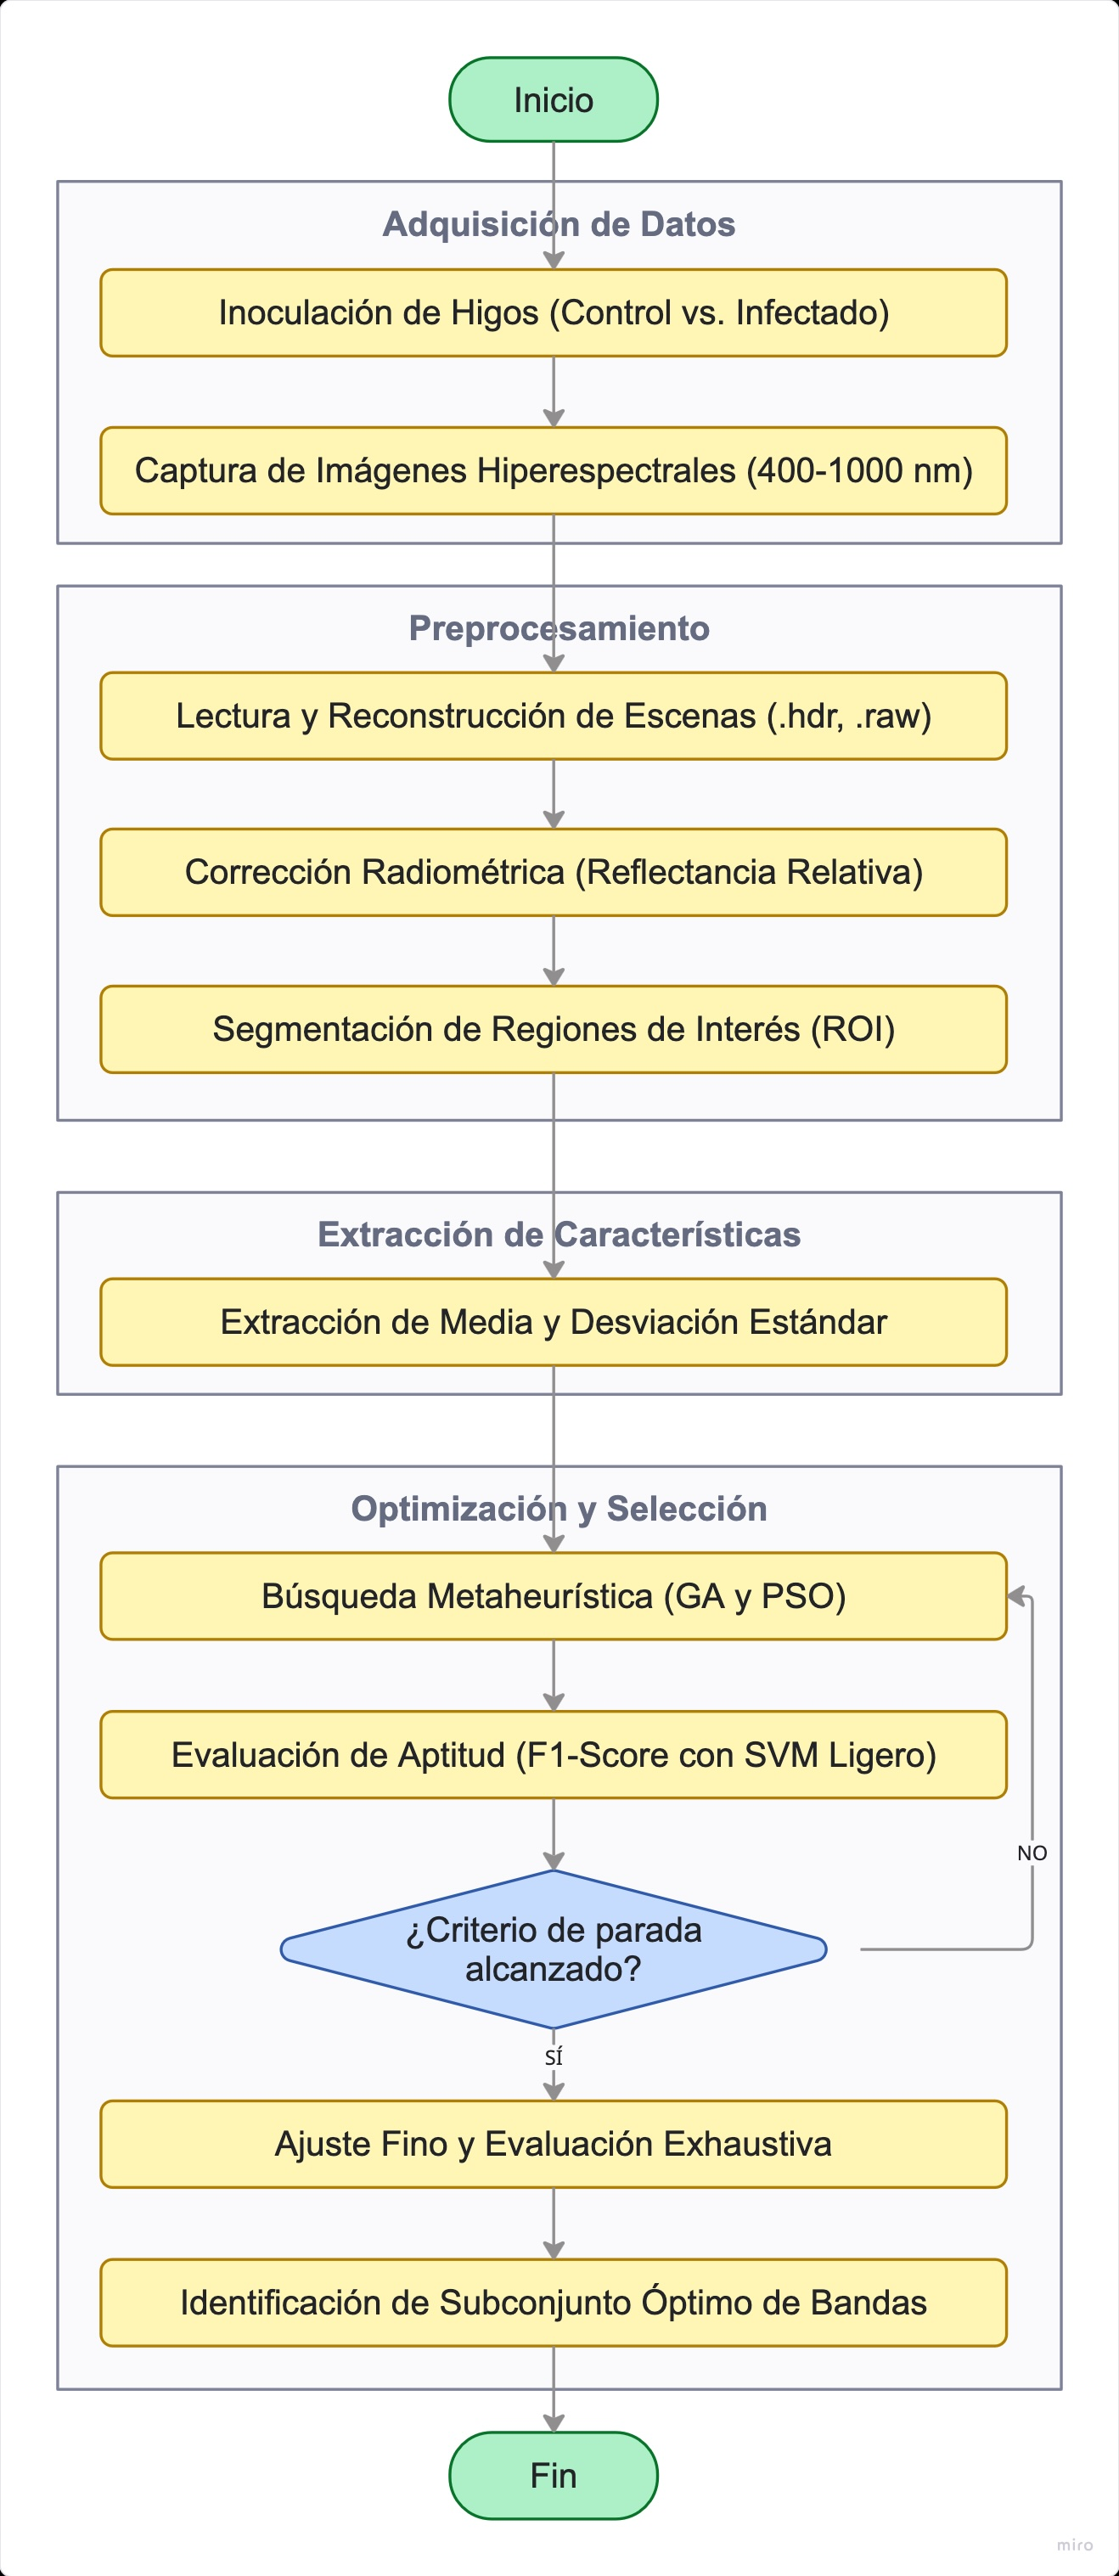
\includegraphics[width=0.6\textwidth]{metodology_flow_chart.jpg}
    \caption{Diagrama de flujo de la metodología computacional propuesta}
    \label{fig:metodologia_flowchart}
\end{figure}

\section{Adquisición de Datos e Inoculación}
\subsection{Material Biológico y Procedencia}
Para el desarrollo de esta investigación, se utilizaron muestras de higos frescos (Ficus carica L.) correspondientes a la variedad Calabacita. Con el fin de garantizar la uniformidad fisiológica del lote de estudio, todas las muestras fueron recolectadas simultáneamente en la "Finca La Orden-Valdesequera", una instalación agro-tecnológica operada por el Centro de Investigaciones Científicas y Tecnológicas de Extremadura (CICYTEX), ubicada en la región de Guadajira, Badajoz, España.

\subsection{Diseño Experimental y Proceso de Inoculación}
El protocolo de inoculación fue ejecutado bajo condiciones controladas de laboratorio por ingenieros agrícolas del CICYTEX. Para el diseño del experimento, la población total de frutos se distribuyó en cuatro bandejas independientes, albergando cada una entre 36 y 40 higos. Una de estas bandejas se mantuvo libre de patógenos para fungir como el grupo de control sano (Clase 0).

Las muestras de las tres bandejas restantes fueron sometidas a un proceso de inoculación artificial, el cual consistió en sumergir la porción inferior de cada fruto durante un lapso de 4 a 5 segundos en una solución fúngica. Se utilizó específicamente la cepa Aspergillus flavus HG 144M, provista por la colección del grupo de investigación CAMIALI de la Universidad de Extremadura.
Para evaluar la progresión de la enfermedad, las soluciones se prepararon en tres concentraciones distintas: $10^3 UFC/ml$, $10^5 UFC/ml$ y $10^7 UFC/ml$. Sin embargo, para los alcances del presente trabajo computacional, centrado en la clasificación binaria, el conjunto de datos de trabajo se construyó utilizando únicamente el grupo de control sano (Clase 0) y el grupo inoculado con la infección más severa de $10^7 UFC/ml$ (Clase 1).

\subsection{Condiciones de Incubación y Monitoreo Temporal}
Entre las sesiones de adquisición de imágenes, las muestras reposaron en una cámara de incubación bajo un ambiente estrictamente controlado. La cámara se configuró para mantener una temperatura constante de 25°C y una humedad relativa de entre 80\% y 90\%, proporcionando las condiciones ambientales óptimas para la proliferación fúngica.

El monitoreo de las muestras se realizó mediante la captura de imágenes hiperespectrales cada 24 horas durante un periodo de cinco días consecutivos posteriores a la inoculación. La adquisición se efectuó empleando una cámara hiperespectral line-scan (pushbroom) modelo SPECIM FX10. El sensor de este dispositivo captura la reflectancia en el rango espectral visible e infrarrojo cercano (VNIR, 400 nm a 1000 nm), ofreciendo una resolución espectral de 448 bandas y una resolución espacial de 1024 píxeles de ancho por cada línea de escaneo \cite{cruz-carrasco_detection_2024}.

\section{Preprocesamiento de Imágenes}
El procesamiento de los datos espaciales y espectrales, así como la extracción inicial de características, se llevó a cabo apoyándose en la biblioteca Spectral Python (SPy) para la manipulación y análisis algorítmico de los cubos hiperespectrales. Como primer paso en el flujo de trabajo, se procedió a la lectura e interpretación de los archivos de encabezado (.hdr) y los archivos de datos binarios (.raw) generados por el sensor SPECIM FX10, lo que permitió reconstruir digitalmente las escenas adquiridas.
Como primer paso en el flujo de trabajo, se procedió a la lectura e interpretación de los archivos de encabezado (.hdr) y los archivos de datos binarios (.raw) generados por el sensor SPECIM FX10, lo que permitió reconstruir digitalmente las escenas adquiridas.

Dado que los valores capturados inicialmente por la cámara representan intensidades lumínicas brutas, las cuales están inherentemente sujetas a fluctuaciones de la fuente de iluminación y al ruido térmico del sensor, fue indispensable aplicar una corrección radiométrica. Los valores de intensidad bruta se convirtieron a reflectancia relativa aplicando referencias claras y oscuras adquiridas junto con cada escena, de acuerdo con la siguiente ecuación\cite{morales_laboratory_2022}:
\begin{equation}
    R=\dfrac{I_{raw}-I_{dark}}{I_{white}-I_{dark}}
\end{equation}

Donde $I_{raw}$ corresponde a la intensidad de la imagen bruta, $I_{dark}$ representa la referencia oscura (capturada con el obturador cerrado para medir la corriente oscura del sensor), e $I_{white}$ es la referencia blanca (obtenida mediante un panel de calibración de reflectancia máxima).

Posterior a la calibración, y con el fin de procesar la información espectral de cada fruto de manera individualizada y libre del ruido de fondo, se procesaron un total de 18 escenas hiperespectrales completas. El aislamiento espacial de las Regiones de Interés (ROI) se efectuó a través de una segmentación manual utilizando el software de anotación de código abierto LabelMe (v5.8.3)\cite{wada_wkentarolabelme_2021}.
Este meticuloso proceso dio como resultado la generación de 560 máscaras de segmentación individuales. Consecuentemente, el conjunto de datos de trabajo final quedó constituido por estas 560 muestras independientes, distribuidas en 277 muestras pertenecientes a la clase de control sana (Clase 0) y 283 muestras correspondientes a la clase inoculada con la concentración severa (Clase 1).

\begin{figure}[H]
    \centering
    \subfloat[]{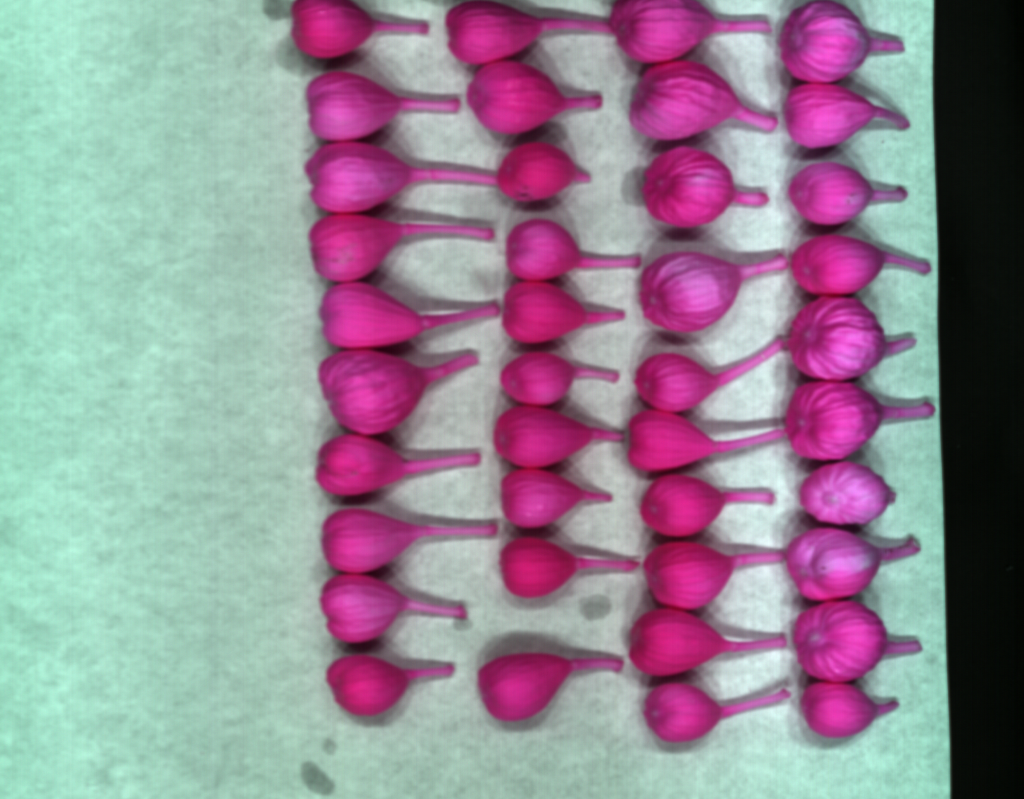
\includegraphics[width=0.4\textwidth]{sample_figs_tray.png}}
    \hspace{1mm}
    \subfloat[]{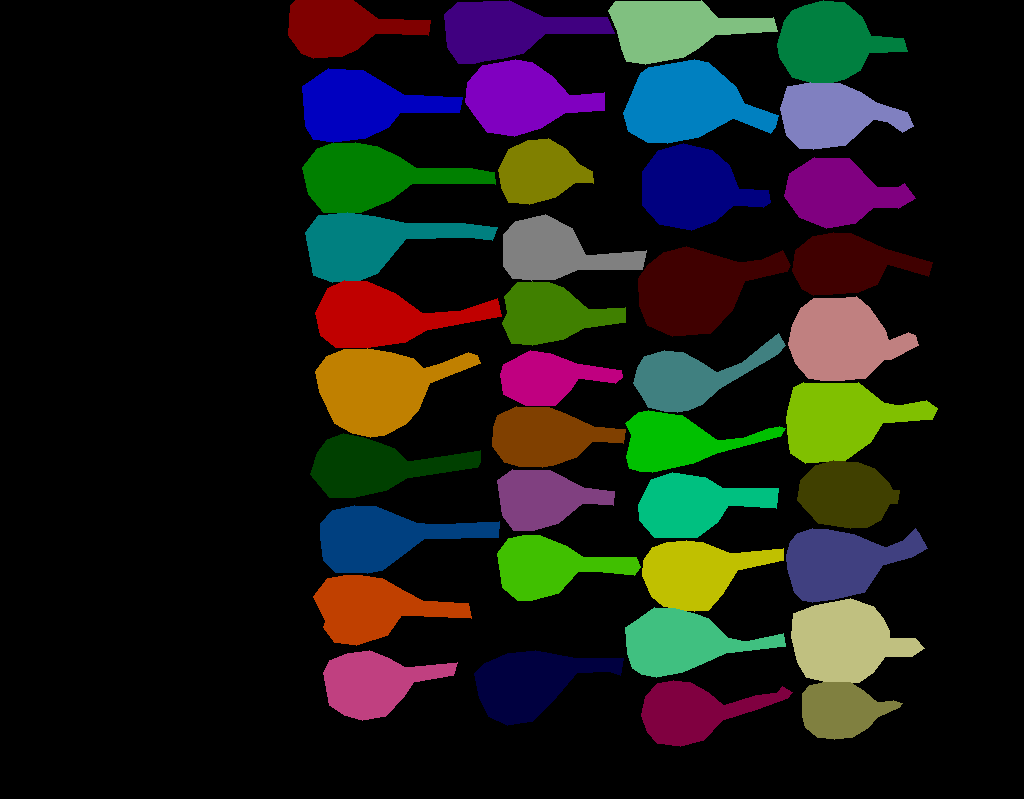
\includegraphics[width=0.4\textwidth]{sample_figs_masks.png}}
    \caption{Charola de higos antes de la segmentación (a) y mascaras de higos después de la segmentación (b)}
    \label{fig:segmentacion}
\end{figure}

\section{Extracción de Características y Construcción del Vector}
La información contenida en las imágenes hiperespectrales es masiva y altamente redundante entre bandas contiguas. Para modelar el problema de clasificación, fue necesario transformar los datos puros de los píxeles dentro de cada Región de Interés (ROI) en descriptores matemáticos \cite{sawant_survey_2020}.
Esta característica conlleva a la llamada \textit{maldición de la dimensionalidad} o fenomeno de Hughes, donde la presición de la clasificación tienede a decrecer conforme el número de bandas espectrales se incrementa dado un número limitado de muestras de entrenamiento \cite{hughes_mean_1968}.

Con el objetivo de capturar tanto el impacto fisiológico interno (cambios en la pigmentación y contenido de agua) como las alteraciones en la textura superficial del fruto, se diseñó una estrategia de construcción de características basada en dos momentos estadísticos:

\begin{enumerate}
    \item Reflectancia Media ($\mu$): Caracteriza la tendencia central de la firma espectral, indicando la cantidad de luz promedio que el tejido absorbe o refleja en una longitud de onda específica \cite{nagasubramanian_hyperspectral_2018}.
    \item Desviación Estándar ($\sigma$): Cuantifica la variabilidad espacial o heterogeneidad en la superficie del fruto. Esta métrica es de suma importancia biológica, ya que la infección por Aspergillus flavus no es uniforme; la formación de micelio y la esporulación alteran la rugosidad superficial del higo, generando patrones de dispersión de luz irregulares que son capturados por esta medida de dispersión \cite{hossain_color_2019}.
\end{enumerate}

Formalmente, para una imagen hiperespectral con n bandas (donde $n=448$), el conjunto completo de características extraídas para la $i$-ésima muestra se definió mediante el siguiente vector concatenado:
\begin{equation}
    X_i=[\mu_i,1,\ldots \mu_i,n,\sigma_i,1,\ldots,\sigma_i,n]
\end{equation}

Este enfoque generó un vector inicial de 896 dimensiones por muestra (448 medias y 448 desviaciones estándar). Para mitigar la maldición de la dimensionalidad, el espacio de búsqueda de optimización se estructuró como un problema de selección de bandas.
Bajo este esquema, la selección de una banda específica j implica la inclusión simultánea e indisoluble de su media ($\mu_j$) y su desviación estándar ($\sigma_j$).
Por lo tanto, el algoritmo metaheurístico opera sobre un espacio de búsqueda binario de n dimensiones (donde 1 indica selección y 0 exclusión), pero la dimensionalidad real del vector de características que evalúa el clasificador es de $ 2\times{k} $, siendo $k$ el número objetivo de bandas seleccionadas ($k\in\{3, 5, 6\}$).

El problema de optimización se definió formalmente como la búsqueda del vector binario $B=\{b1,...,bn\}$ que maximice la función de aptitud, se estableció el F1-Score como la función objetivo a maximizar:

\begin{equation}
    F1=2 \times{\frac{Precision\times{Recall}}{Precision+Recall}}
\end{equation}

Se eligio el F1-Score como la función de aptitud debido a su habilidad para balancear presición y sensibilidad. Es critico penalizar falsos negativos (higos infectados clasificados erroneamente como sanos), ya que representan un alto riesgo para la salud. Ademas, el F1-Score provee una métrica robusta ya que mitiga efectivamente el sesgo potencial introducido por la pequeña diferencia entre la cantidad de higos en Clase 0 y la Clase 1 en el conjunto de datos.

\section{Proceso de Optimización (Diseño Metaheurístico)}
\begin{itemize}
    \item Se implementaron GA y PSO para buscar un vector binario que maximice el rendimiento de clasificación, con tamaños de subconjuntos objetivo de 3, 5 y 6 bandas \cite{eiben_introduction_2015}.
    \item Para mitigar la carga computacional iterativa, se diseñó una estrategia de evaluación en dos etapas: 
    \begin{itemize}
        \item \textbf{Evaluador rápido:} Un modelo SVM ligero configurado para estimar la aptitud de los individuos rápidamente y guiar la búsqueda del algoritmo \cite{nagasubramanian_hyperspectral_2018}.
        \item \textbf{Evaluador exhaustivo:} Un ajuste fino de hiperparámetros utilizado únicamente sobre el mejor subconjunto encontrado al final de la optimización \cite{nagasubramanian_hyperspectral_2018}. Antes del entrenamiento, los datos fueron normalizados con StandardScaler.
    \end{itemize}
\end{itemize}

\chapter{Experimentación y Resultados}

\section{Medidas y Métricas Utilizadas}
Para evaluar la aptitud funcional de las bandas seleccionadas, la métrica elegida fue el F1-Score. Esta medida es fundamental porque balancea la precisión y la sensibilidad, penalizando rigurosamente los falsos negativos (clasificar un higo infectado como sano), un escenario que representa un riesgo inaceptable para la seguridad alimentaria \cite{cruz-carrasco_detection_2024}.
\begin{equation}
    F1=2 \times{\frac{Precision\times{Recall}}{Precision+Recall}}
\end{equation}

\section{Configuraciones Experimentales}
Ambos algoritmos metaheurísticos fueron ejecutados de manera independiente 30 veces para cada tamaño de subconjunto objetivo ($k \in \{3, 5, 6\}$) \cite{eiben_introduction_2015}. En las siguientes tablas se muestran las configuraciones del GA, PSO y SVM respectivamente:

\begin{table}[H] 
%\small % Change table font size
\caption{Parametros del Algoritmo Genético.\label{tab:ga_params}}
%\isPreprints{\centering}{} % Only used for preprints
\begin{tabularx}{\textwidth}{CCCCC}
\toprule
\textbf{Generaciones} & \textbf{Tamaño de población} & \textbf{Tipo de selección} & \textbf{Cruza} & \textbf{Tasa de mutación}\\
\midrule
350 & 250 & Torndeo de 2 & Cruza de un punto & 2.5\\
\bottomrule
\end{tabularx}
\noindent
\end{table}

\begin{table}[H] 
%\small % Change table font size
\caption{Parametros de PSO.\label{tab:pso_params}}
%\isPreprints{\centering}{} % Only used for preprints
\begin{tabularx}{\textwidth}{CCCCCC}
\toprule
\textbf{Iteraciones} & \textbf{Particulas} & \textbf{Coeficiente cognitivo (C1)} & \textbf{Coeficiente social (C2)} & \textbf{Inercia} & \textbf{Tasa de mutación}\\
\midrule
650 & 200 & 0.4 a 2.5 & 2.5 a 0.4 & 0.7 & 0.2\\
\bottomrule
\end{tabularx}
\noindent
\end{table}

\begin{table}[H] 
%\small % Change table font size
\caption{Parametros de SVM.\label{tab:svm_params}}
%\isPreprints{\centering}{} % Only used for preprints
\begin{tabularx}{\textwidth}{CCCCC}
\toprule
\textbf{Implementación} & \textbf{Kernel} & \textbf{regularización ($C$)} & \textbf{Gamma ($\gamma$)} & \textbf{Método de validación}\\
\midrule
Fast evaluator       & RBF & Fixed 1.0             & Fixed scale & k-fold CV ($k=3$)\\ \\
Exhaustive evaluator & RBF & Grid search 0.1 a 1000 & Grid search 0.001 a 1 & k-fold CV ($k=5$)\\
\bottomrule
\end{tabularx}
\noindent
\end{table}

\section{Caracterización Espectral de las Muestras}
Como paso previo a la evaluación del rendimiento de los algoritmos de clasificación y optimización, se realizó un análisis exploratorio del comportamiento espectral de las muestras en el rango VNIR (400 nm a 1000 nm). Este análisis es fundamental para comprender la naturaleza de los datos y justificar la pertinencia de las características extraídas.

La Figura \ref{fig:mean_std_reflectance} ilustra las firmas espectrales promedio de reflectancia tanto para la clase de frutos sanos (control) como para la clase con infección severa por Aspergillus flavus. Las regiones sombreadas representan la desviación estándar, ilustrando la dispersión de los datos dentro de cada clase. Como se puede observar, los patrones espectrales de ambas clases presentan una similitud visual extremadamente alta, evidenciando un solapamiento casi total en la región del espectro visible (400 - 700 nm). Se aprecia una divergencia sutil en la intensidad de reflectancia únicamente en la región del infrarrojo cercano (NIR, 700 - 1000 nm), un fenómeno atribuible a la degradación de la estructura celular interna del tejido del higo inducida por la colonización fúngica. Este alto grado de solapamiento espectral confirma la complejidad intrínseca de la tarea de clasificación y justifica la necesidad de emplear técnicas avanzadas de selección de bandas en lugar de umbrales espectrales simples.

Sin embargo, el análisis de la variabilidad espacial revela un comportamiento diametralmente distinto. La Figura 5.1b presenta la desviación estándar de la reflectancia en función de la longitud de onda para ambas clases. En esta representación, se evidencia de manera contundente que las muestras infectadas exhiben una variabilidad espacial (textural) consistentemente superior en comparación con los higos sanos a lo largo de todo el espectro.

Esta evidencia empírica respalda la hipótesis central de la metodología propuesta: la infección fúngica, altera la heterogeneidad en la superficie del higo. Por lo tanto, se confirma que la inclusión de la desviación estándar ($\sigma$) en el vector de características no es redundante, sino que aporta información discriminatoria crítica que la reflectancia media ($\mu$) por sí sola es incapaz de capturar.

\begin{figure}[H]
\centering
\subfloat[\centering]{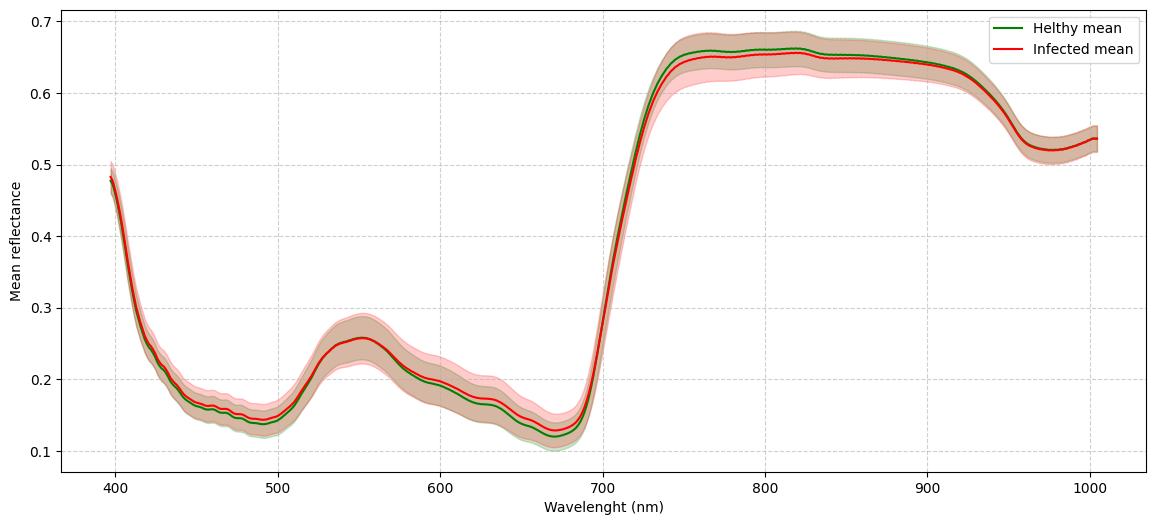
\includegraphics[width=13.0cm]{Imagenes/spectral_signature_mean_reflectance.png}}\\
\subfloat[\centering]{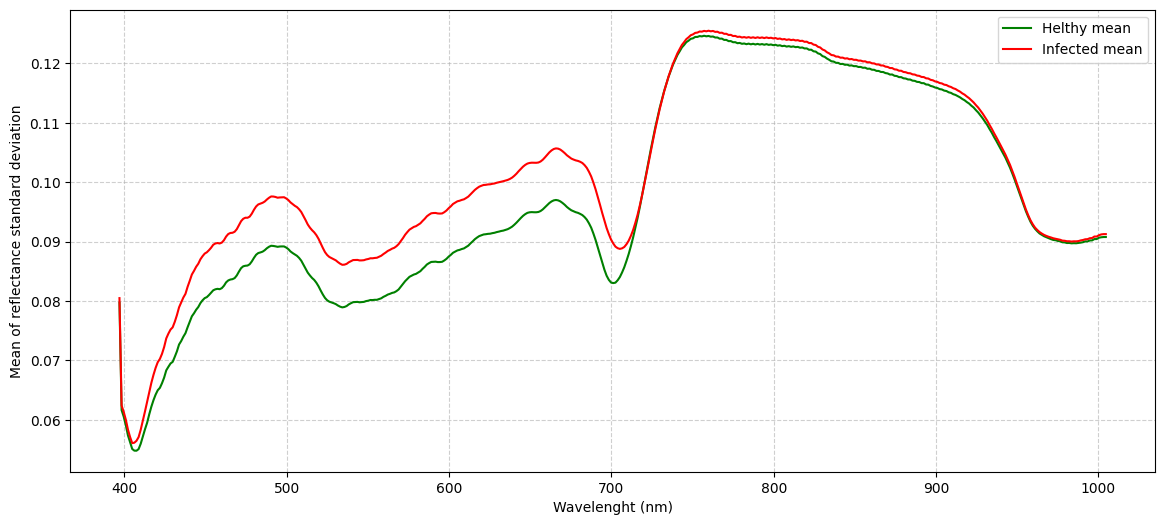
\includegraphics[width=13.0cm]{Imagenes/spectral_signature_mean_standard_deviation.png}}
\caption{Caracterización espectral de las muestras de higo. (\textbf{a}) Firmas de reflectancia media mostrando la tendencia central. (\textbf{b}) Desviación estándar de la reflectancia representando la variabilidad espacial (textura).\label{fig:mean_std_reflectance}}
\end{figure} 

\section{Resultados}
Una vez confirmada la relevancia espectral de las características extraídas, se procedió a evaluar el rendimiento cuantitativo de los algoritmos metaheurísticos en la tarea de reducción de dimensionalidad y clasificación.

\subsection{Resultados de la Construcción de Características}
El primer experimento tuvo como objetivo validar computacionalmente la hipótesis planteada en la sección anterior: la superioridad del vector de características combinado ($\mu + \sigma$) sobre el uso exclusivo de la reflectancia media ($\mu$).
Para ello, se ejecutó el proceso de selección de bandas bajo ambas configuraciones, estableciendo tamaños de subconjuntos objetivo de $k \in\{3, 5, 6\}$ a lo largo de 30 ejecuciones independientes.

Los resultados, promediados y presentados en la Tabla \ref{tab:ga_performance}, demuestran que la inclusión de la desviación estándar mejora significativamente la exactitud del modelo. Incrementando la métrica \textit{F1-Score} particularment en los subconjuntos de menor dimensionalidad, alcanzando una mejora del $+9.2\%$ para $k=3$ y del $+7.2\%$ para $k=5$
\begin{table}[H] 
%\small % Change table font size
\caption{Comparación de desempeño GA (F1-Score promedio) entre características.\label{tab:ga_performance}}
%\isPreprints{\centering}{} % Only used for preprints
\begin{tabularx}{\textwidth}{CCCC}
\toprule
\textbf{Tamaño de individuo} & \textbf{Solo media de reflectancia ($\mu$)} & \textbf{Características combinadas ($\mu + \sigma$)} & \textbf{Mejora (\%)} \\
\midrule
3 Bandas & 0.663 & 0.755 & +9.2\% \\
5 Bandas & 0.698 & 0.77  & +7.2\% \\
6 Bandas & 0.721 & 0.773 & +5.2\%  \\
\bottomrule
\end{tabularx}
\noindent
\end{table}

Adicionalmente, el análisis del historial de convergencia del Algoritmo Genético (Figura \ref{fig:ga_convergence}) confirma que la estrategia combinada no solo inicia con una aptitud superior desde las primeras generaciones, sino que mantiene una trayectoria de optimización mucho más robusta. Esto sugiere que la información textural estabiliza el espacio de búsqueda, permitiendo a la metaheurística eludir mínimos locales y converger hacia soluciones de mayor calidad con mayor eficiencia.
\begin{figure}[H]
%\begin{adjustwidth}{-\extralength}{0cm}
\centering
\subfloat[\centering]{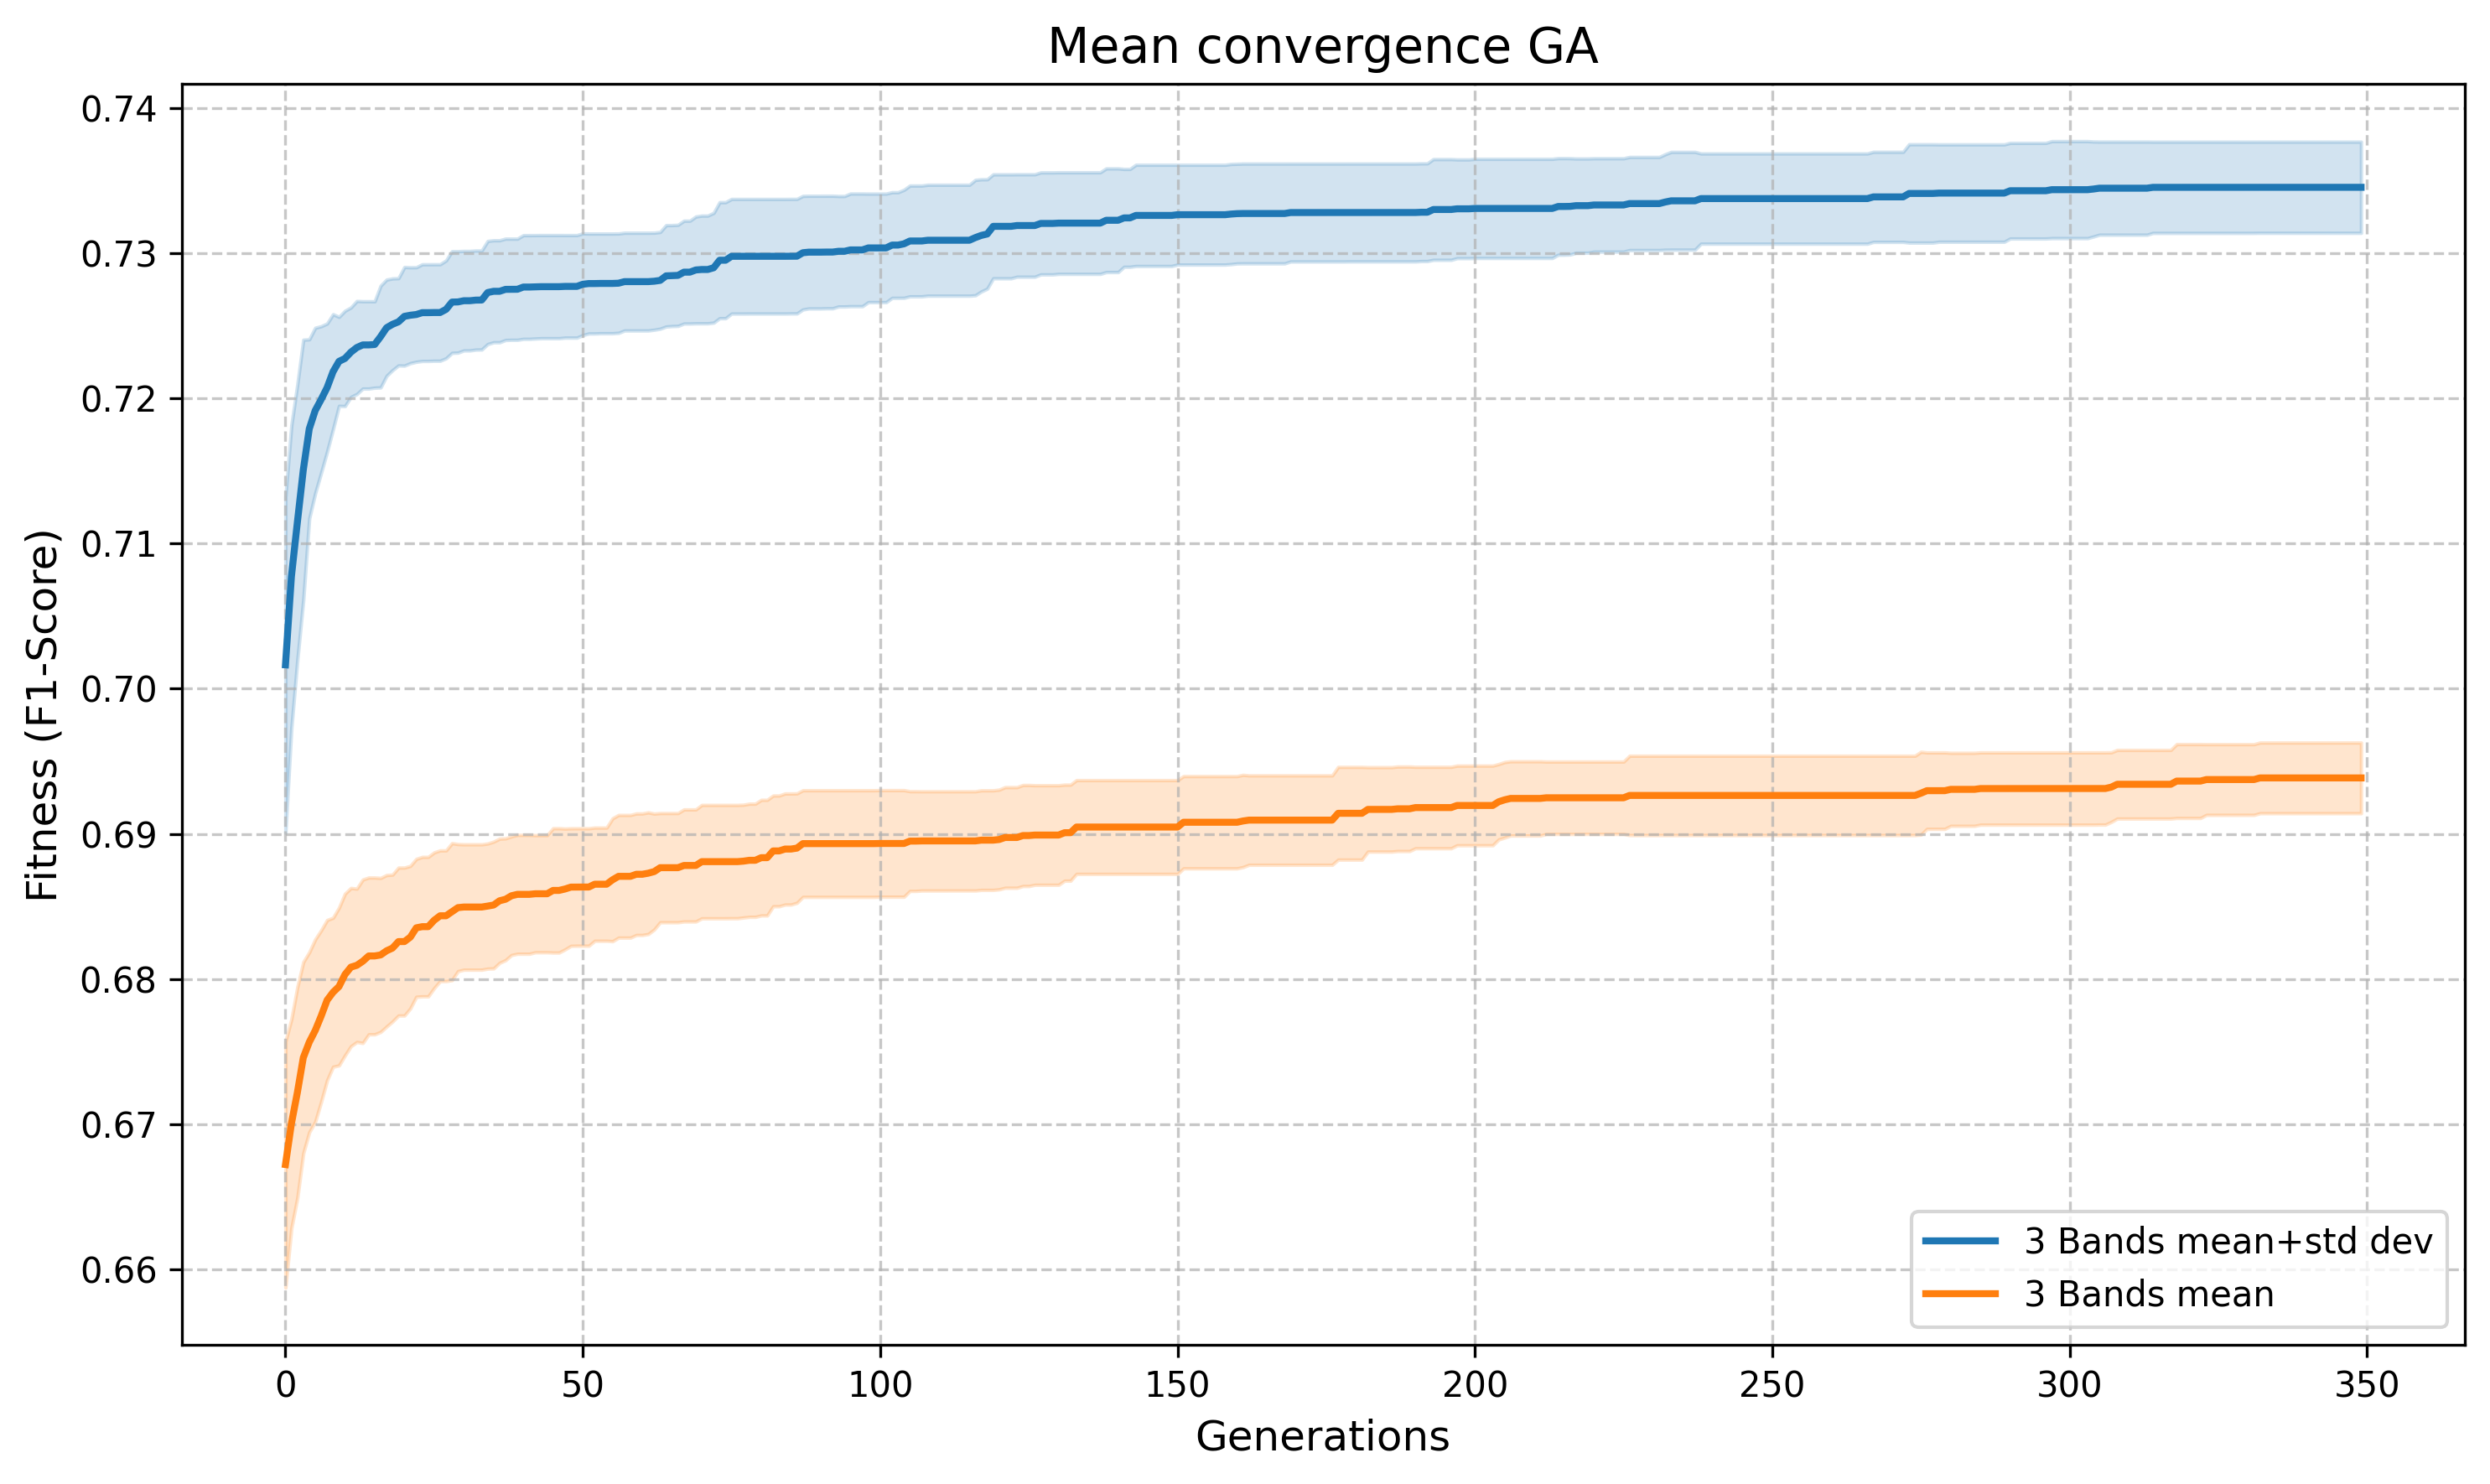
\includegraphics[width=8.2cm]{Imagenes/mean_convergence_3b.png}} 
%\hfill
\subfloat[\centering]{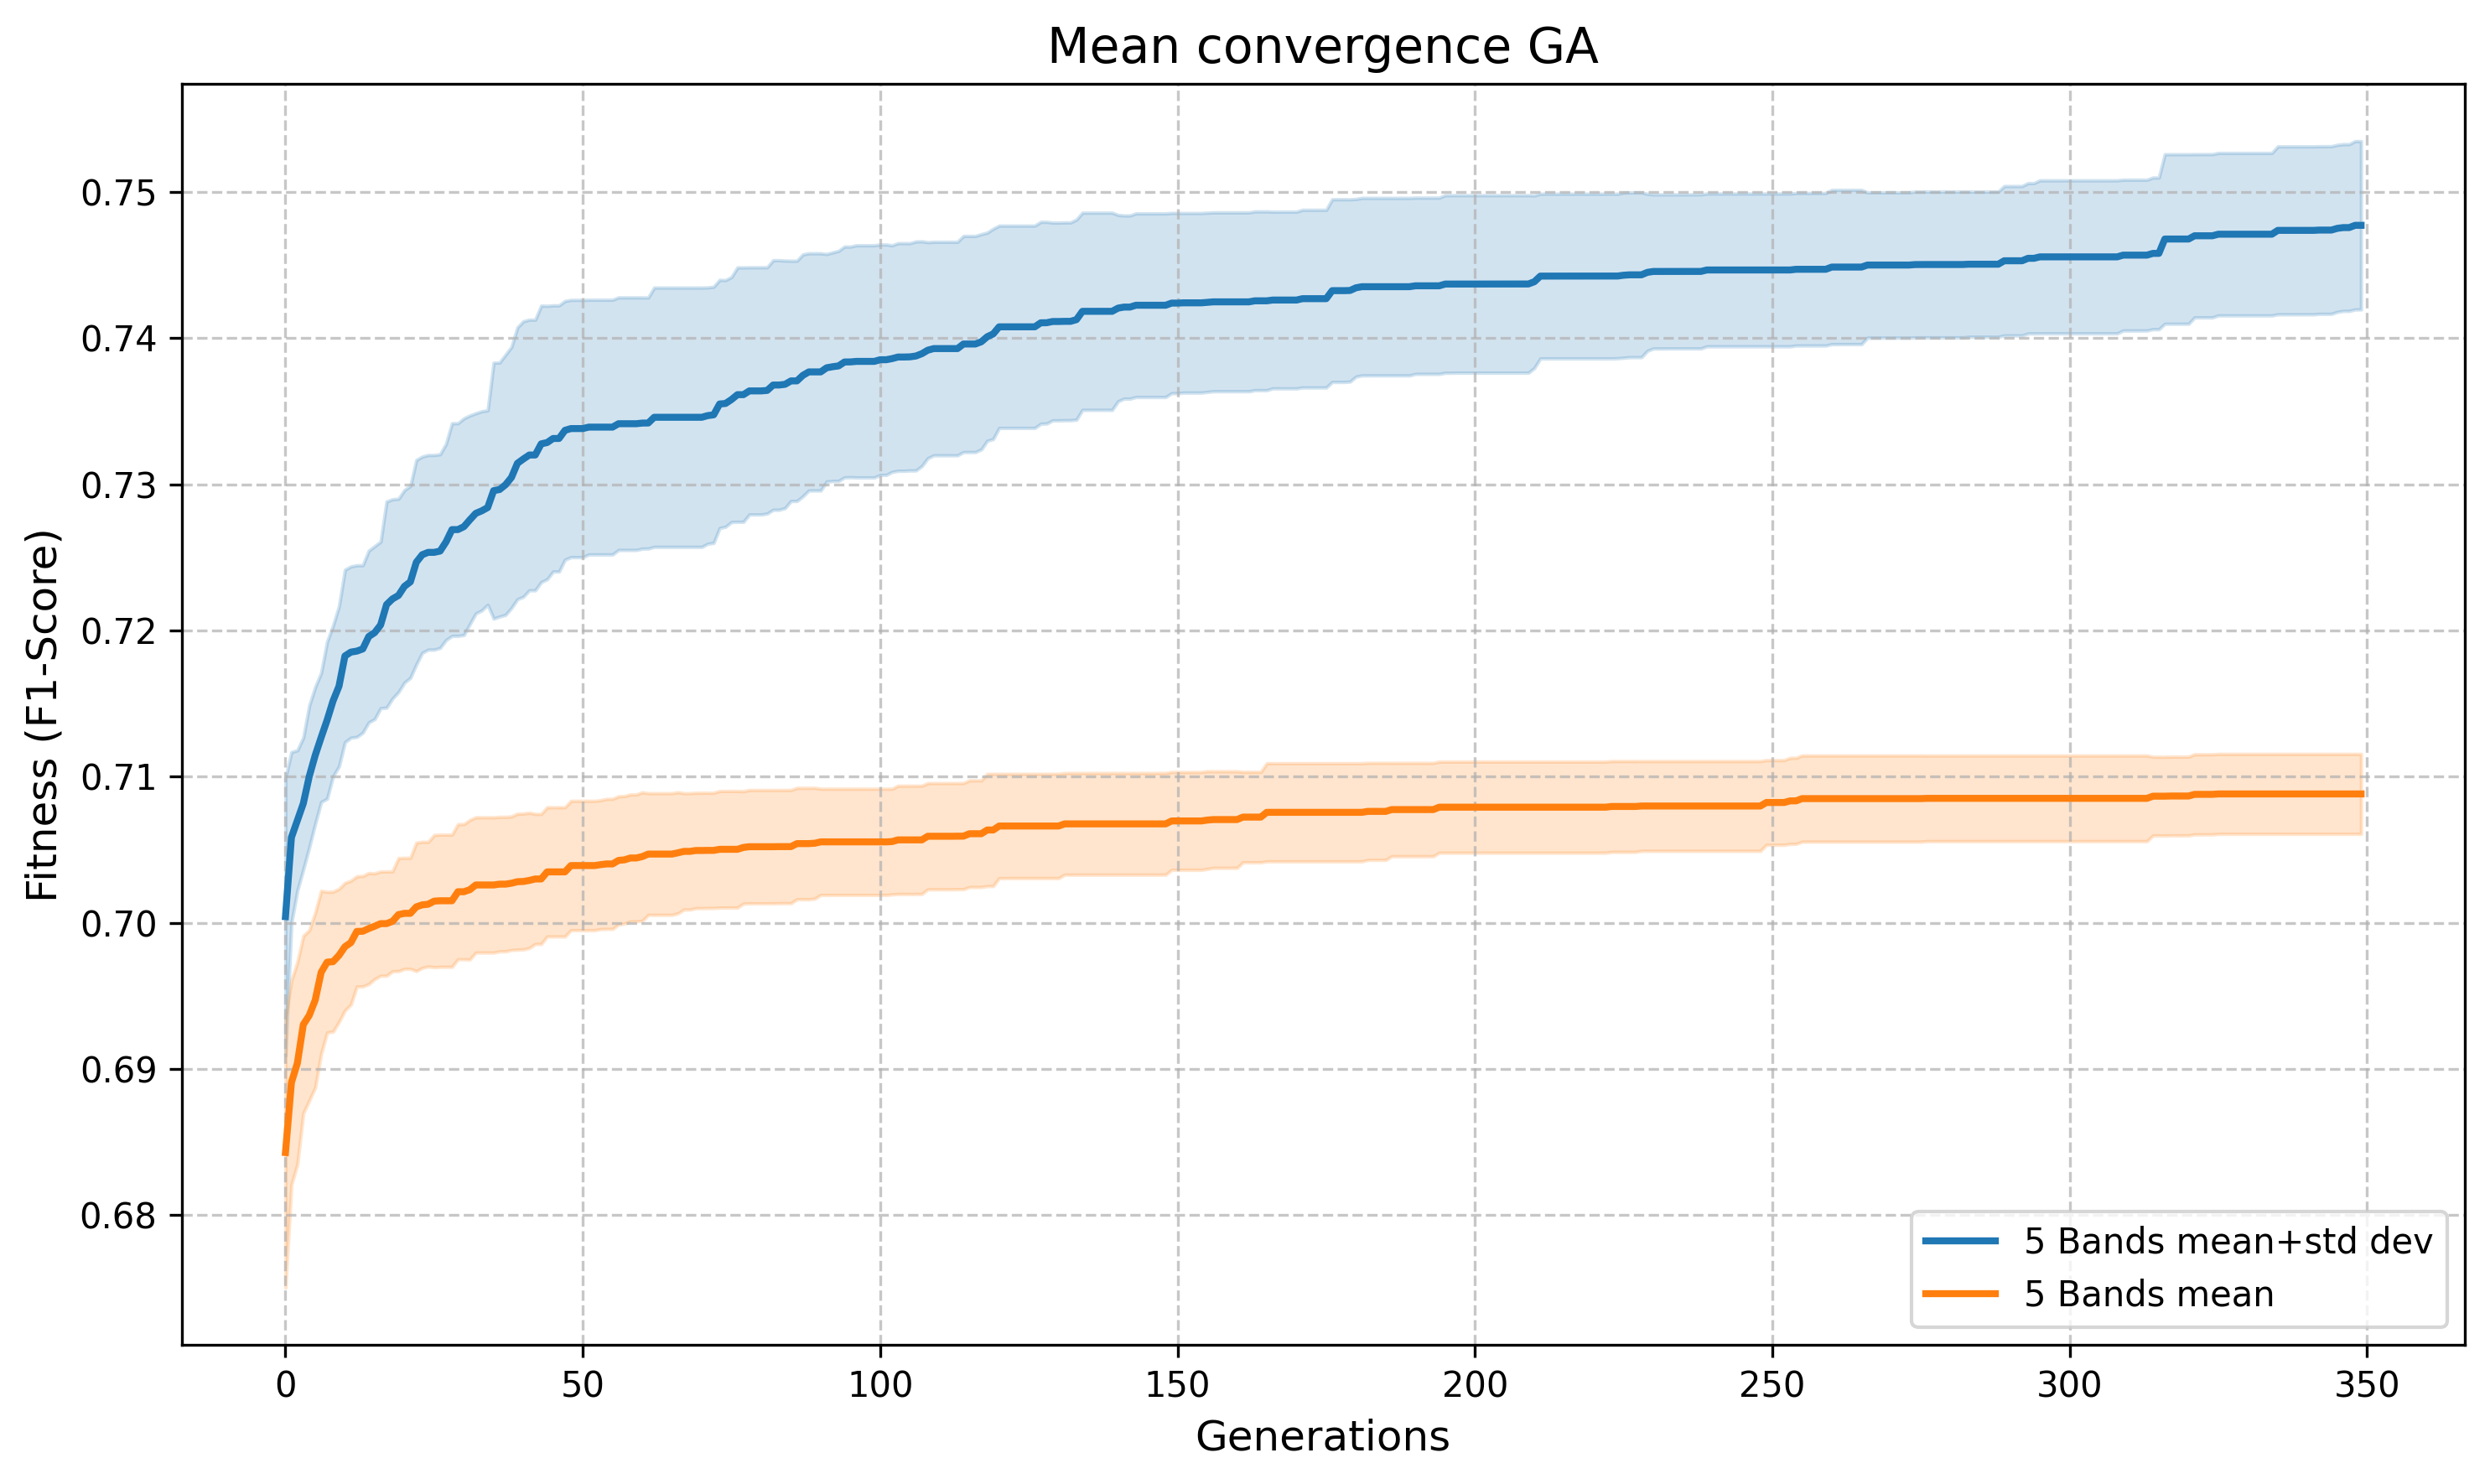
\includegraphics[width=8.2cm]{Imagenes/mean_convergence_5b.png}}\\
\subfloat[\centering]{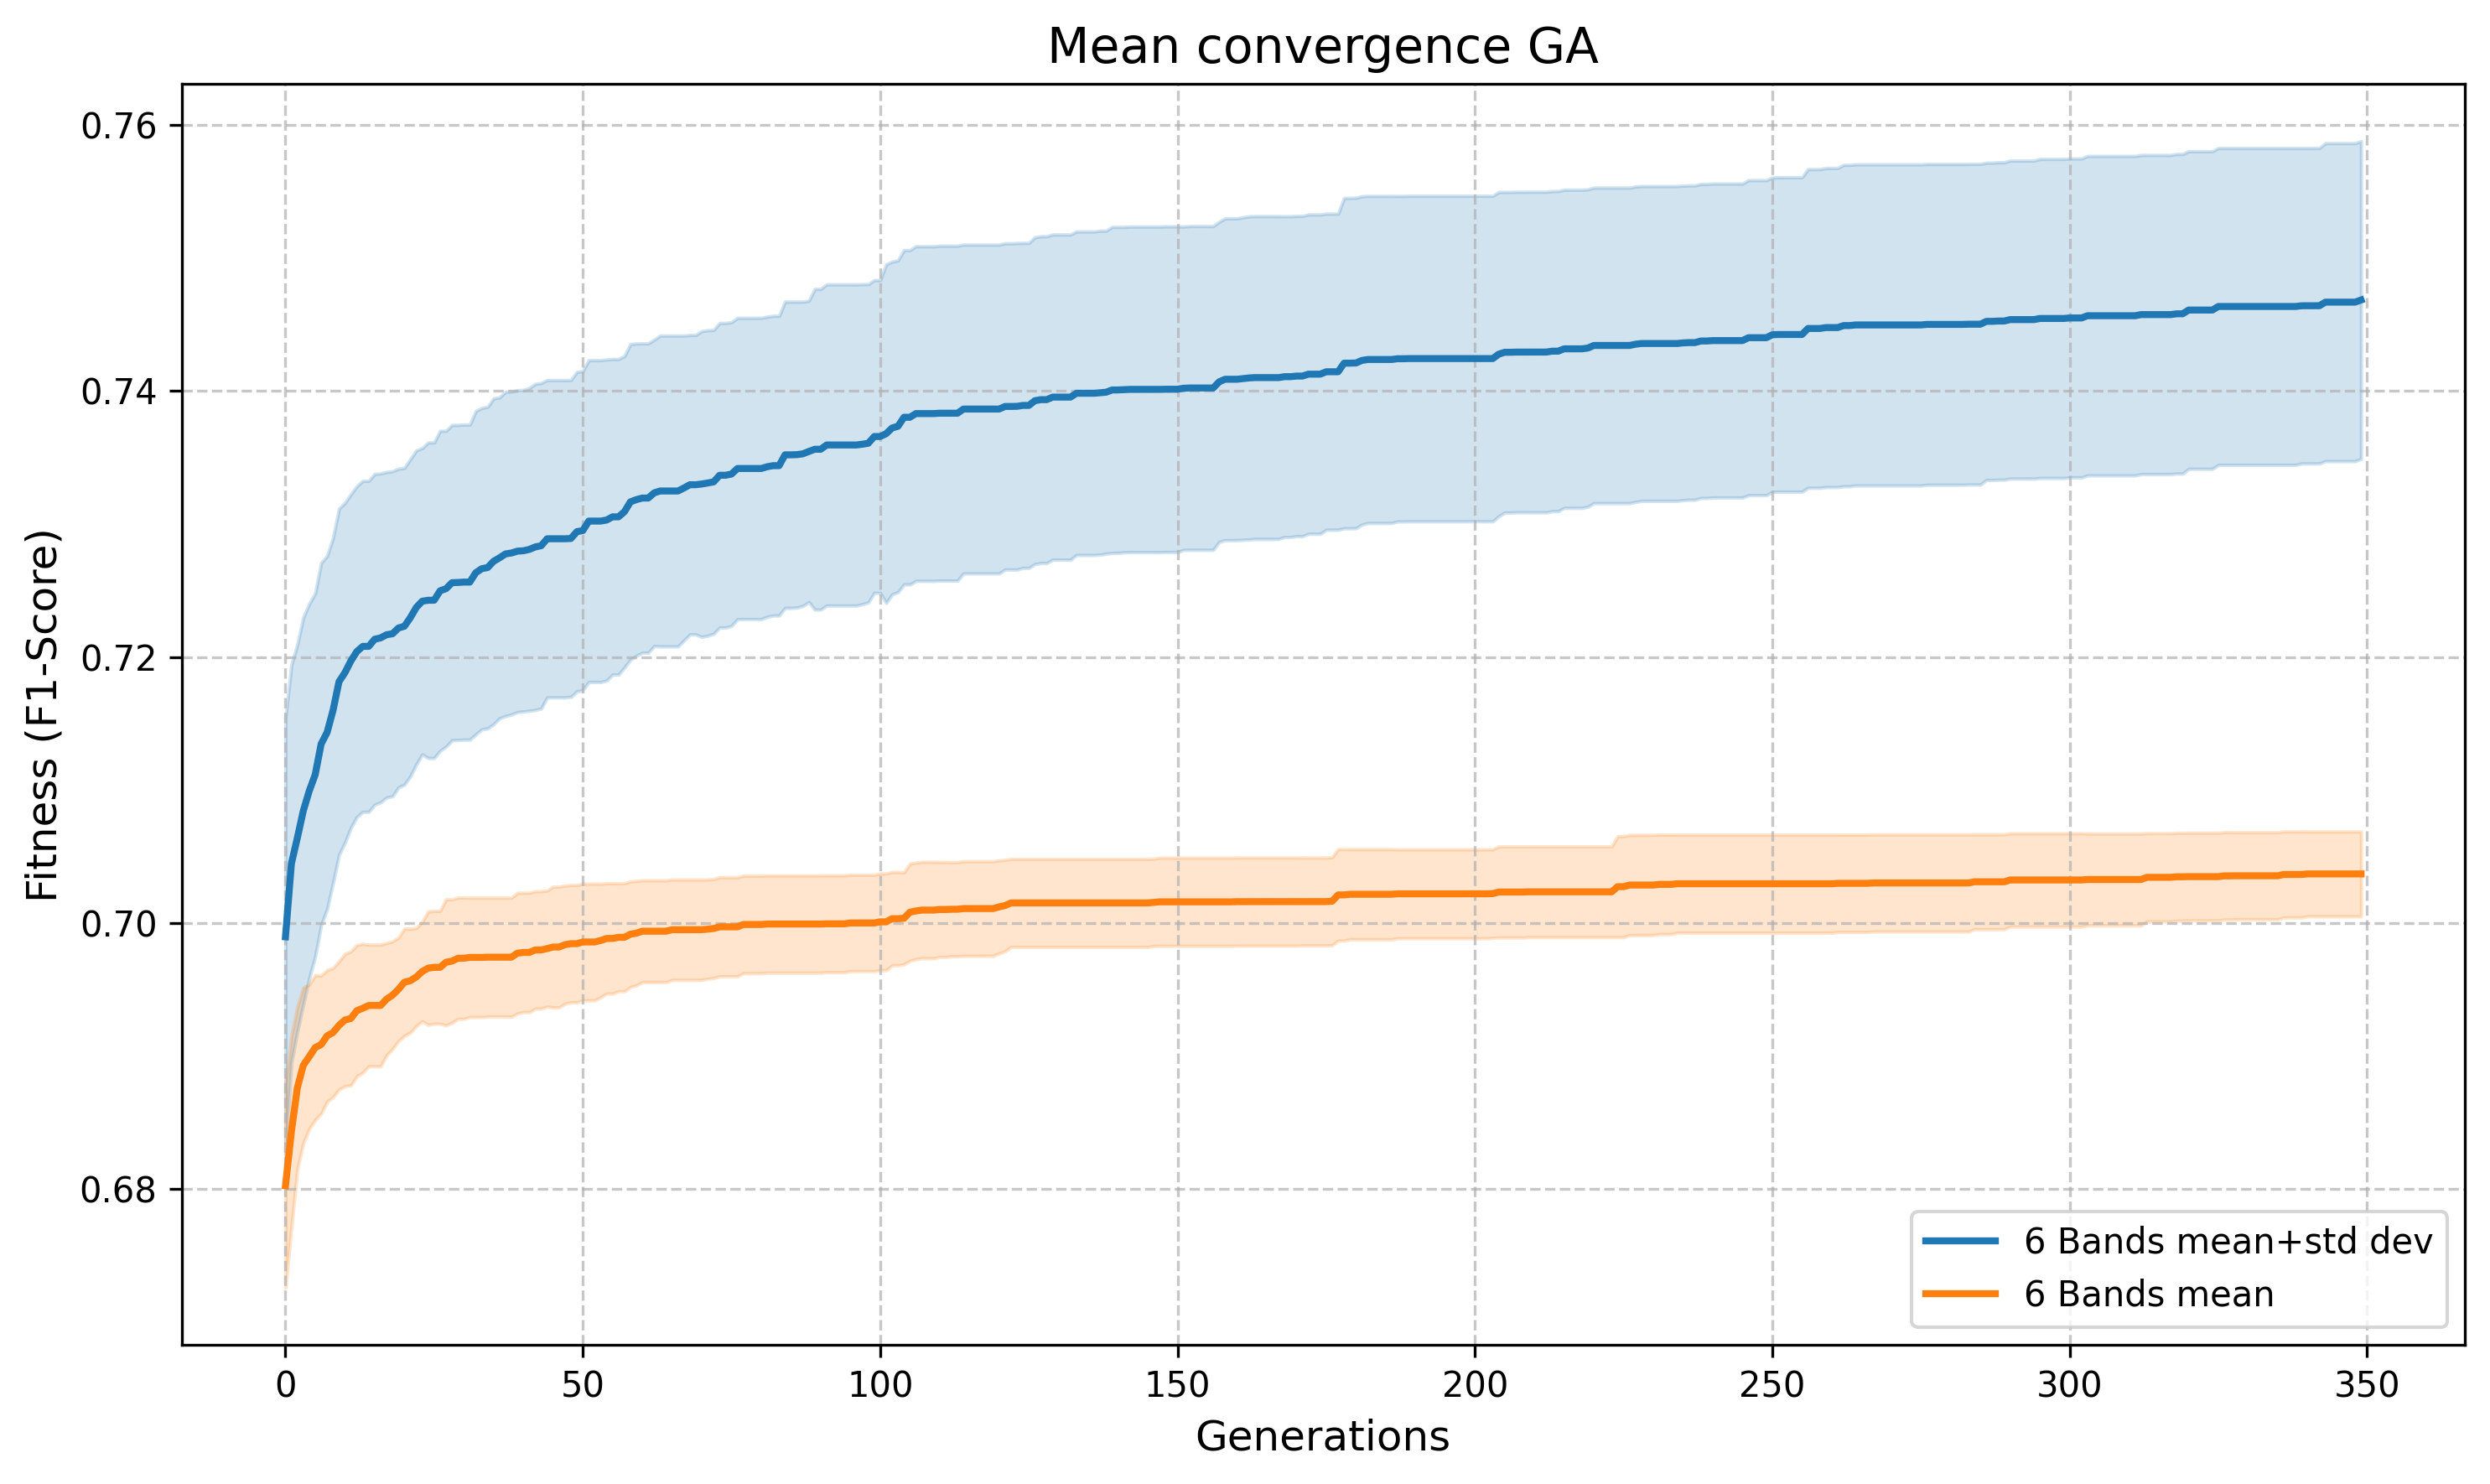
\includegraphics[width=8.2cm]{Imagenes/mean_convergence_6b.png}}
\hfill
%\end{adjustwidth}
%\caption{Convergence history of the Genetic Algorithm over 30 independent runs. (\textbf{a}) 3 bands optimization. (\textbf{b}) 5 bands optimization. (\textbf{c}) 6 bands optimization.\label{fig:4}}
\caption{Media de convergencia de las ejecuciones del algoritmo genetico durante 30 ejecuciones independientes para los escenarios: (\textbf{a}) 3 Bandas; (\textbf{b}) 5 Bandas; y (\textbf{c}) 6 Bandas.\label{fig:ga_convergence}}
\end{figure} 

\subsection{Análisis Comparativo del Rendimiento: GA y PSO}
Tras validar la construcción del vector, el segundo análisis se enfocó en contrastar las capacidades de optimización global del Algoritmo Genético frente a la Optimización por Enjambre de Partículas. La distribución estadística de los valores F1-Score obtenidos tras 30 ejecuciones independientes se resume mediante diagramas de caja en la Figura \ref{fig:boxplot_ga_pso}.
\begin{figure}[H]
\centering
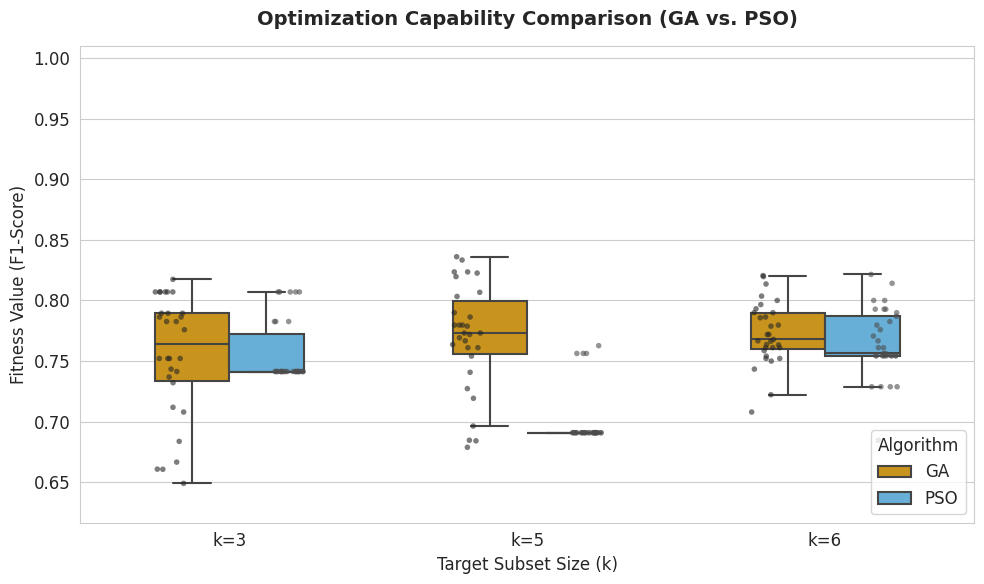
\includegraphics[width=12.0 cm]{Imagenes/boxplot_comparison_mean_std.png}
\caption{Diagrama de cajas: comparación de GA vs. PSO con características ($\mu+\sigma$).}
\label{fig:boxplot_ga_pso}
\end{figure}   
\unskip
\hfill \break

\begin{figure}[H]
\centering
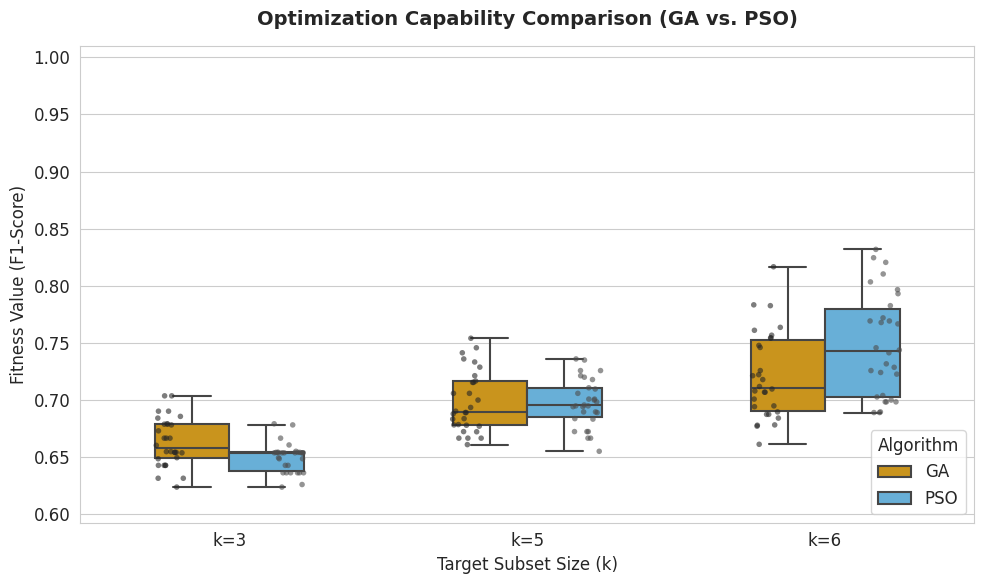
\includegraphics[width=12.0 cm]{Imagenes/boxplot_comparison_mean.png}
\caption{Diagrama de cajas: comparación de GA vs. PSO únicamente con media ($\mu$).}
\label{fig:boxplot_ga_pso_mean}
\end{figure}   
\unskip

El análisis comparativo revela que ambas metaheurísticas son altamente competentes para la selección de bandas hiperespectrales, aunque presentan sutiles diferencias en su comportamiento. El GA demostró una consistencia general ligeramente superior, exhibiendo una mediana de F1-Score más alta y rangos intercuartílicos más estrechos para los subconjuntos de 5 y 6 bandas. Esta menor dispersión indica una mayor estabilidad algorítmica y reproducibilidad en sus resultados.

Por otro lado, el algoritmo PSO mostró una ligera ventaja competitiva en el escenario más restrictivo (3 bandas). Más importante aún, el PSO fue el algoritmo capaz de encontrar el óptimo absoluto global de todo el estudio: un F1-Score máximo de 0.836 utilizando la configuración de 5 bandas combinadas. Este hallazgo subraya la excelente capacidad de explotación local que otorgan los Coeficientes de Aceleración Variables en el Tiempo (TVAC) implementados en el PSO.

En conclusión, los resultados validan que es posible reducir drásticamente la dimensionalidad de los datos hiperespectrales (pasando de cientos de bandas a un conjunto óptimo de cinco) sin sacrificar la precisión diagnóstica para la detección de Aspergillus flavus, sentando un precedente viable para la implementación de futuros sistemas de inspección agrícola.
\chapter{Conclusiones \label{cap:Conclusiones}}

// Este capítulo resume las contribuciones de tu ICR, puede separarse en secciones como: aportación al estado del arte, aportación al área de investigación. Por último, esboza direcciones futuras de la ICR.





\appendix
\include{Anexos/Anexo1}
%\include{Anexos/Anexo2}


% \backmatter
\addcontentsline{toc}{chapter}{Bibliografía}
\bibliographystyle{unsrt}
\nocite{*}
\bibliography{Referencias/Referencias}

\end{document}

